\subsection{Antecedentes SRGAN}


Como se menciona las CNN<

Las GAN´s (Generative Adversarial Networks) son un tipo de redes cuyo funcionamiento está basado
en la estimación de modelos generadores, como mencionan Goodfellow et al. \cite{GANs}, esto es 
posible gracias al entrenamiento de un modelo \emph{generador (G)} que obtiene la distribución de 
los datos y un modelo \emph{discriminador (D)} el cual se encarga de estimar la probabilidad 
de que la muestra provenga del dataset de entrenamiento en lugar del modelo generador \emph{G}.

\begin{figure}[H]
    \begin{center}
      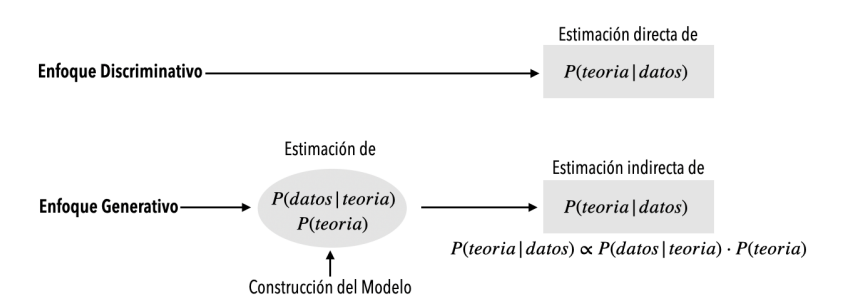
\includegraphics[width=12cm,height=8cm]{modelo_gen_disc.png}
      \caption{Modelo Generador y Discriminador}
      \label{Alex1}
    \end{center}
    \end{figure}